\iffalse
\title{2023-ME}
\author{EE24BTECH11020 -  Ellanti Rohith}
\section{me}
\chapter{2023}
\fi
\item He did not manage to fix the car himself, so he \underline{\hspace{2cm}} in the garage.
    
    \hfill{[GATE 2023]}\begin{enumerate}
    \begin{multicols}{2}
        \item got it fixed
        \item getting it fixed
        \item gets fixed
        \item got fixed
        \end{multicols}
    \end{enumerate}

     \item Planting : Seed :: Raising : \underline{\hspace{2cm}} \\
    (By word meaning)

    \hfill{[GATE 2023]}\begin{enumerate}
    \begin{multicols}{2}
        \item Child
        \item Temperature
        \item Height
        \item Lift
        \end{multicols}
    \end{enumerate}


\item A certain country has 504 universities and 25951 colleges. These are categorized into Grades I, II, and III as shown in the given pie charts.\\ What is the percentage, correct to one decimal place, of higher education institutions (colleges and universities) that fall into Grade III?

\begin{center}
    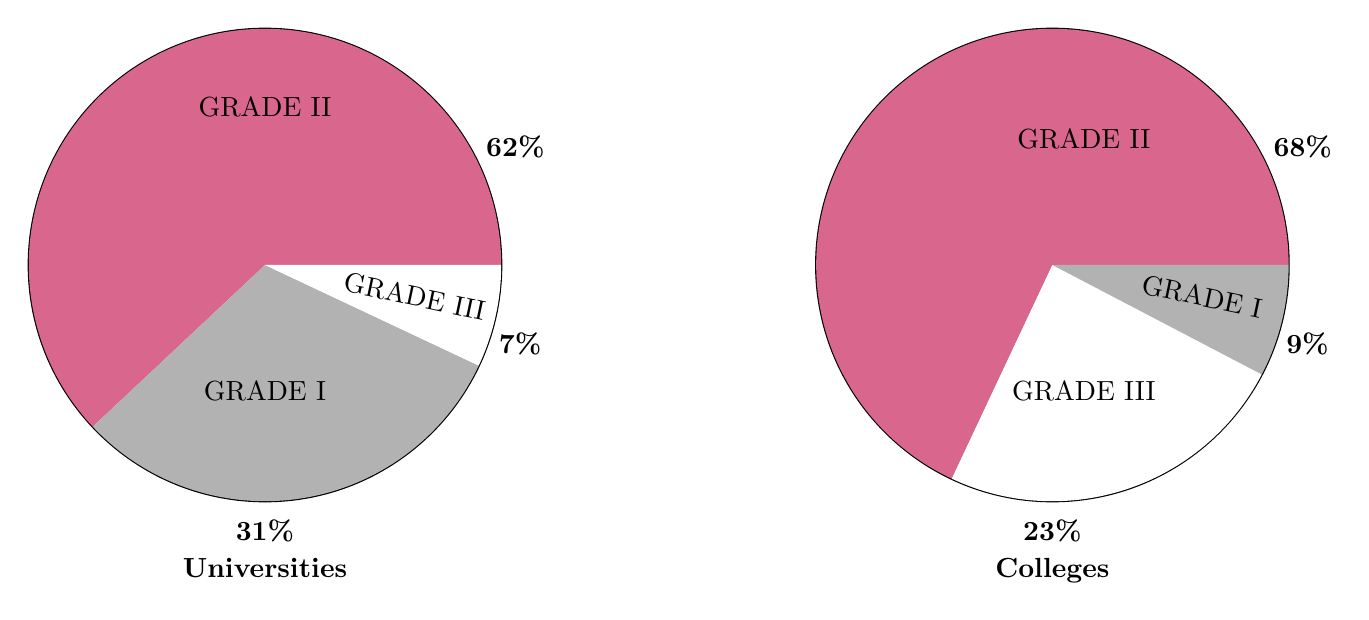
\begin{tikzpicture}[scale=2]  
        \begin{scope}
        \draw[thick] (0,0) circle (1.5cm);         
            \fill[purple!60] (0,0) -- (0:1.5) arc[start angle=0, end angle=223.2, radius=1.5] -- cycle;
            \node at (1.59,0.75) {\textbf{62\%}};
             \node at (1.62,-0.5) {\textbf{7\%}};
            \node at (0,1) {GRADE II};         
            \fill[gray!60] (0,0) -- (223.2:1.5) arc[start angle=223.2, end angle=334.8, radius=1.5] -- cycle;
            \node at (0,-1.69) {\textbf{31\%}};
            \node at (0,-0.8) {GRADE I};
\fill[white] (0,0) -- (334.8:1.5) arc[start angle=334.8, end angle=360, radius=1.5] -- cycle;
\node[rotate=-12] at (0.95,-0.2) {GRADE III};
            \node[below] at (0, -1.8) {\textbf{Universities}};
        \end{scope}
\begin{scope}[xshift=5cm]         
\draw[thick] (0,0) circle (1.5cm);    
            \fill[purple!60] (0,0) -- (0:1.5) arc[start angle=0, end angle=244.8, radius=1.5] -- cycle;
          \fill[white] (0,0) -- (244.8:1.5) arc[start angle=244.8, end angle=332.4, radius=1.5] -- cycle;
          \fill[gray!60] (0,0) -- (332.4:1.5) arc[start angle=332.4, end angle=360, radius=1.5] -- cycle;
           \node at (1.62,-0.5) {\textbf{9\%}}; 
\node at (0,-1.69) {\textbf{23\%}};
\node at (1.59,0.75) {\textbf{68\%}};
            \node at (0.2,-0.8) {GRADE III};
             \node at (0.2,0.8) {GRADE II};
\node[rotate=-12] at (0.95,-0.2) {GRADE I};

            \node[below] at (0, -1.8) {\textbf{Colleges}};
        \end{scope}

    \end{tikzpicture}
\end{center}

\hfill{[GATE 2023]}\begin{enumerate}

\begin{multicols}{4}
   \item 22.7
   \item 23.7
   \item 15.0
   \item 66.8

    \end{multicols}
\end{enumerate}
\item The minute-hand and second-hand of a clock cross each other \underline{\hspace{1.5cm}} times between 09:15:00 AM and 09:45:00 AM on a day.


\hfill{[GATE 2023]}\begin{enumerate}
\begin{multicols}{4}
    \item 30
    \item 15
    \item 29
    \item 31
    \end{multicols}
\end{enumerate}

\item The symbols $ \circ $, $ \ast $, $ \triangle $, and $ \square $ are to be filled, one in each box, as shown below.

The rules for filling in the four symbols are as follows.

\begin{enumerate}
    \item Every row and every column must contain each of the four symbols.
    \item Every $2 \times 2$ square delineated by bold lines must contain each of the four symbols.
\end{enumerate}

 Which symbol will occupy the box marked with ? in the partially filled figure?
\begin{figure}[!ht]
\centering
\resizebox{0.3\textwidth}{!}{%
\begin{circuitikz}
\tikzstyle{every node}=[font=\large]
\draw [ line width=1.2pt](3.75,11.75) to[short] (3.75,6.75);
\draw [ line width=1.2pt](3.75,6.75) to[short] (8.75,6.75);
\draw [ line width=1.2pt](8.75,11.75) to[short] (8.75,6.75);
\draw [ line width=1.2pt](3.75,11.75) to[short] (8.75,11.75);
\draw [line width=1.2pt, dashed] (5,11.75) -- (5,6.75);
\draw [line width=1.2pt, dashed] (7.5,11.75) -- (7.5,6.75);
\draw [line width=1.2pt, dashed] (3.75,10.5) -- (8.75,10.5);
\draw [line width=1.2pt, dashed] (3.75,8) -- (8.75,8);
\draw [ line width=1.2pt](6.25,11.75) to[short] (6.25,6.75);
\draw [ line width=1.2pt](3.75,9.25) to[short] (8.75,9.25);
\node [font=\large] at (4.35,7.25) {$\ast$};
\node [font=\large] at (7,9.9) {$\ast$};
\node [font=\large] at (8.1,8.5) {$\ast$};
\node [font=\large] at (8.25,11) {$\triangle$};
\node [font=\large] at (7,7.35) {$\triangle$};
\node [font=\large] at (5.7,9.8) {$\circ$};
\node [font=\large] at (8.1,7.25) {$\circ$};
\node [font=\large] at (7,8.5) {$\square$};
\node [font=\large] at (5.7,11) {$?$};
\end{circuitikz}
}%

\end{figure}
\hfill{[GATE 2023]}\begin{enumerate}

\begin{multicols}{2}
    \item $ \circ $
    \item $ \ast $
    \item $ \triangle $
    \item $ \square $
    \end{multicols}
\end{enumerate}

\item In a recently held parent-teacher meeting, the teachers had very few complaints about Ravi. After all, Ravi was a hardworking and kind student. Incidentally, almost all of Ravi's friends at school were hardworking and kind too. But the teachers drew attention to Ravi's complete lack of interest in sports. The teachers believed that, along with some of his friends who showed similar disinterest in sports, Ravi needed to engage in some sports for his overall development.

Based only on the information provided above, which one of the following statements can be logically inferred with \textbf{certainty}?

\hfill{[GATE 2023]}\begin{enumerate}
    \item All of Ravi's friends are hardworking and kind.
    \item No one who is not a friend of Ravi is hardworking and kind.
    \item None of Ravi's friends are interested in sports.
    \item Some of Ravi's friends are hardworking and kind.
\end{enumerate}
 \item Consider the following inequalities
\begin{align*}
    p^2 - 4q &< 4 \\
    3p + 2q &< 6
\end{align*}
where $ p $ and $ q $ are positive integers.\\
The value of $ \brak{p + q} $ is \underline{\hspace{2cm}}.

\vspace{1em}

\hfill{[GATE 2023]}\begin{enumerate}\begin{multicols}{4}
    \item 2
    \item 1
    \item 3
    \item 4
    \end{multicols}
\end{enumerate}
\item Which one of the sentence sequences in the given options creates a coherent narrative?

\begin{enumerate}
    \item[(i)] I could not bring myself to knock.
    \item[(ii)] There was a murmur of unfamiliar voices coming from the big drawing room and the door was firmly shut.
    \item[(iii)] The passage was dark for a bit, but then it suddenly opened into a bright kitchen.
    \item[(iv)] I decided I would rather wander down the passage.
\end{enumerate}

\vspace{1em}


\hfill{[GATE 2023]}\begin{enumerate}
\begin{multicols}{2}
   \item (iv), (i), (iii), (ii)
   \item (iii), (i), (ii), (iv)
   \item (ii), (i), (iv), (iii)
   \item (i), (iii), (ii), (iv)
    \end{multicols}
\end{enumerate}
\item How many pairs of sets (S, T) are possible among the subsets of $ \{1, 2, 3, 4, 5, 6\} $ that satisfy the condition that $ S $ is a subset of $ T $?
\hfill{[GATE 2023]}
\begin{multicols}{2}
\begin{enumerate}
   \item 729
   \item 728
   \item 665
   \item 664
\end{enumerate}
\end{multicols}

\item An opaque pyramid (shown below), with a square base and isosceles faces, is suspended in the path of a parallel beam of light, such that its shadow is cast on a screen oriented perpendicular to the direction of the light beam. The pyramid can be reoriented in any direction within the light beam. Under these conditions, which one of the shadows \textbf{P, Q, R}, and \textbf{S} is \textbf{NOT} possible?
\begin{center}
\resizebox{0.3\textwidth}{!}{%
\begin{circuitikz}
\tikzstyle{every node}=[font=\large]
\fill[lightgray] (6.25,8.75) -- (7.75,10.25) -- (6.25,11.75) --(4.5,10) --cycle;
\draw [black, line width=1.2pt](6.25,11.75) to[short] (6.25,8.75);
\draw [black, line width=1.2pt](6.25,11.75) to[short] (7.75,10.25);
\draw [black, line width=1.2pt](6.25,8.75) to[short] (7.75,10.25);
\draw [black, line width=1.2pt](6.25,11.75) to[short] (4.5,10);
\draw [black, line width=1.2pt](4.5,10) to[short] (6.25,8.75);
\draw [black, line width=1.2pt, dashed] (4.5,10) -- (6.55,10.3);
\draw [black, line width=1.2pt, dashed] (6.25,11.75) -- (6.55,10.3);
\draw [black, line width=1.2pt, dashed] (6.55,10.3) -- (7.75,10.25);



\end{circuitikz}
}%
\end{center}\begin{enumerate}
\begin{multicols}{2}
\item

\resizebox{0.25\textwidth}{!}{%
\begin{circuitikz}
\tikzstyle{every node}=[font=\normalsize]

\filldraw[fill=gray!30, draw=black] 
    ((0,0)--(1.5,0)--(2,-0.5)--(1.5,-1)--(0,-1) -- cycle;
\node at (1,-0.4) {\textbf{P}};

\end{circuitikz}
}%

\item
\resizebox{0.25\textwidth}{!}{%
\begin{circuitikz}
\tikzstyle{every node}=[font=\normalsize]

\filldraw[fill=gray!30, draw=black] 
    (4,12) -- (5.25,12.75) -- (5.75,12.25) -- (6.75,12.5) -- (6.55,11.5) -- (7.1,11) -- (5.25,10.5) -- cycle;
 \node at (5.5,11.5) {\textbf{Q}};

\end{circuitikz}
}%


\item
\resizebox{0.15\textwidth}{!}{%
\begin{circuitikz}
\tikzstyle{every node}=[font=\normalsize]

\filldraw[fill=gray!30, draw=black] 
    (5,8.25) -- (6.5,9) -- (8,7.75) -- (6.5,5.75) -- cycle;

\node at (6.5,8) {\textbf{R}};

\end{circuitikz}
}%
\item
\resizebox{0.15\textwidth}{!}{%
\begin{circuitikz}
\tikzstyle{every node}=[font=\normalsize]

\filldraw[fill=gray!30, draw=black] 
    (0,1) -- (1,1) -- (1,0) -- (0,0) -- cycle;
 \node at (0.5,0.5) {\textbf{s}};

\end{circuitikz}
}%

\end{multicols}
\end{enumerate}
\hfill{[GATE 2023]}\begin{enumerate}
\begin{multicols}{2}
   \item \textbf{P}
   \item \textbf{Q}
   \item \textbf{R}
   \item \textbf{S}
    \end{multicols}
\end{enumerate}
\item A machine produces a defective component with a probability of 0.015. The number of defective components in a packed box containing 200 components produced by the machine follows a Poisson distribution. The mean and the variance of the distribution are

\hfill{[GATE 2023]}\begin{enumerate}
\begin{multicols}{2}
   \item 3 and 3, respectively
   \item $ \sqrt{3} $ and $ \sqrt{3} $, respectively
   \item 0.015 and 0.015, respectively
   \item 3 and 9, respectively
    \end{multicols}
\end{enumerate}

\item The figure shows the plot of a function over the interval $\sbrak{-4, 4}$. Which one of the options given \textbf{CORRECTLY} identifies the function?\\
\begin{center}
\resizebox{0.4\textwidth}{!}{%
\begin{circuitikz}
\tikzstyle{every node}=[font=\LARGE]
\draw [->, >=Stealth] (1.75,8) -- (11.25,8);
\draw [->, >=Stealth] (6.25,7.5) -- (6.25,11);
\draw (2.25,10) to[short] (4.25,8);
\draw (4.25,8) to[short] (6.25,10);
\draw (6.25,10) to[short] (8.25,8);
\draw (8.25,8) to[short] (10.25,10);
\node at (4.25,8) [circ] {};
\node at (6.25,10) [circ] {};
\node at (8.25,8) [circ] {};
\node at (10,8) [circ] {};
\node at (2.25,8) [circ] {};
\node [font=\LARGE] at (8.25,7.5) {2};
\node [font=\LARGE] at (10,7.5) {4};
\node [font=\LARGE] at (2.25,7.5) {-4};
\node [font=\LARGE] at (4.25,7.5) {-2};
\node [font=\LARGE] at (6.5,7.75) {0};
\node [font=\LARGE] at (5.75,10) {2};
\node [font=\LARGE] at (6,11.5) {$y$};
\node [font=\LARGE] at (11,7.25) {$x$};
\end{circuitikz}
}%
\end{center}

\hfill{[GATE 2023]}\begin{enumerate}
    \begin{multicols}{2}
       \item $ |2 - x| $
       \item $ |2 - |x|| $
       \item $ |2 + |x|| $
       \item $ 2 - |x| $
    \end{multicols}
\end{enumerate}
\item With reference to the Economic Order Quantity (EOQ) model, which one of the options given is correct?\\ 
\begin{center}
\resizebox{0.6\textwidth}{!}{%
\begin{circuitikz}
\tikzstyle{every node}=[font=\large]
\draw (2.5,13) to[short] (2.5,6);
\draw (2.5,6) to[short] (11.25,6);
\draw (11.25,13) to[short] (11.25,6);
\draw [color={rgb,255:red,0; green,128; blue,0}](2.5,6.5) to[short] (11.25,6.5);
\draw [ color={rgb,255:red,255; green,0; blue,0}, dashed] (3,12.75) .. controls (3,9.25) and (5.5,7) .. (11.25,10.5);
\draw [color={rgb,255:red,0; green,0; blue,255}, dashed] (3,12.75) .. controls (3.5,6) and (5.25,7.75) .. (11.5,7);
\draw [ color={rgb,255:red,128; green,0; blue,128}, dashdotted] (2.5,6) -- (11.25,9.75);
\node [font=\large, rotate around={90:(0,0)}] at (2.1,9.5) {$Cost\text{ } per\text{ } unit \rightarrow$};
\node [font=\large] at (7.75,5.5) {$Order\text{ } quantity \rightarrow$};
\node [font=\normalsize, color={rgb,255:red,255; green,0; blue,0}] at (9.25,10.75) {$Curve \, P1$};
\node [font=\normalsize, color={rgb,255:red,128; green,0; blue,128}] at (10.5,8.5) {$Curve \, P2$};
\node [font=\normalsize, color={rgb,255:red,0; green,0; blue,255}] at (8.75,8) {$Curve \, P3$};
\node [font=\normalsize, color={rgb,255:red,0; green,128; blue,0}] at (5.75,7) {$Curve \, P4$};
\draw [->, >=Stealth] (6.5,7) -- (7.75,6.5);
\draw [->, >=Stealth] (9,7.75) -- (9.5,7.25);
\draw [->, >=Stealth] (9.25,10.5) -- (9.5,9.75);
\draw [->, >=Stealth] (10.5,8.75) -- (10,9.25);
\end{circuitikz}
}%
\end{center}


\hfill{[GATE 2023]}\begin{enumerate}
   \item Curve P1: Total cost, Curve P2: Holding cost, Curve P3: Setup cost, and Curve P4: Production cost.
   \item Curve P1: Holding cost, Curve P2: Setup cost, Curve P3: Production cost, and Curve P4: Total cost.
   \item Curve P1: Production cost, Curve P2: Holding cost, Curve P3: Total cost, and Curve P4: Setup cost.
   \item Curve P1: Total cost, Curve P2: Production cost, Curve P3: Holding cost, and Curve P4: Setup cost.
\end{enumerate}

